\chapter{Results}\label{ch:results}

The following section will
present the aptness of GP Regression (gp) to estimate certain target measures.
The target measures are: one-week mean, one-day mean, one-hour mean and time in target
range have been presented.
The estimation performance of GP Regression will be compared to that of some
baseline methods, which are: linear regression (linear),
smoothing splines (spline), overall mean (overall\_mean) and naive ttr (naive\_ttr).

The performance will be reported based on different downsampling factors.
A downsampling factor of 2 implies that the data used for estimation
(training data) contains half of the samples from the original signal $F_X$,
which has 10 samples per hour.
Additionally, results will be presented for uniform as well as seasonal sampling.
%In the latter the training data set would contain samples that where drawn
%with probability weights following the cyclic component of $f(x)$.




\section{One-Week Mean}

Figure \ref{fig:weekly-mean-performance} shows the performance
of different methods to
estimate the one-week mean based on different downsampling patterns.
The performance is presented in the form of CI Width and CI Coverage.
CI Width is the width of the estimated 95\%-CI, for the
one-week mean BP value, and it is provided in mmHg.
The CI coverage is the number of times the true one-week BP values
was covered by the estimated CI over 100 simulations.


The perfect method would reach 95\% CI Coverage with very
low CI Width and would thus be in the left upper corner.
Also reaching the 95\% coverage is deemed more important
than having low width.
CI are additionally provided for the CI Coverage and whenever these
span a region that goes above the 95\% Coverage, the method is deemed adequate.


Note, that all the plots show the same range of CI Coverage values on
the y-Axis, but the x-axis range of CI Width values varies.
As expected the CI Width values increase with larger downsampling factor
and with seasonal sampling. Very large downsampling factors, would
result in very large confidence interval for smoothing spline of over
100 mmHg. The CI Width is hence capped at a value of 30 mmHg also since
that larger CI would hardly be of any value.
The approach used for spline interpolation seems to produce very
unstable estimates during bootstrapping, which leads to very large confidence intervals.

\begin{figure}[!ht]
\centering
\begin{subfigure}{\textwidth}
    \centering
    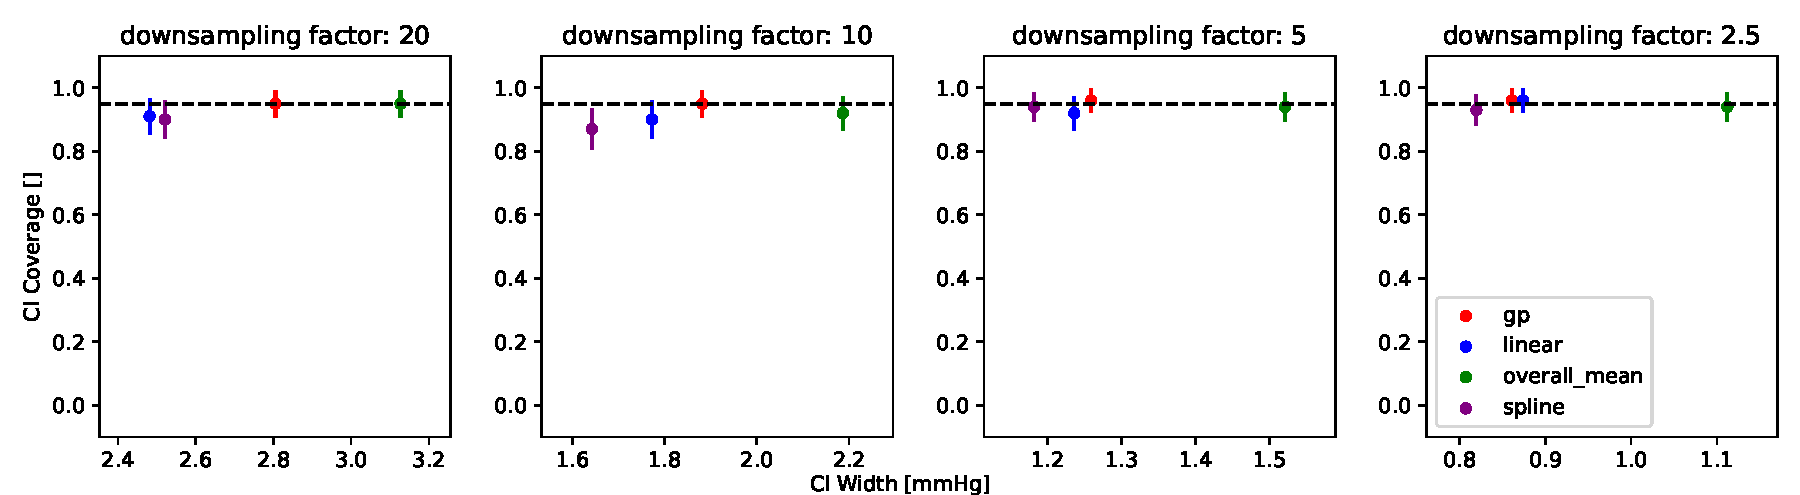
\includegraphics[width=\linewidth]{Pictures/final_experiment_hpdi/overall_mean_eval_sin_rbf_default}
    \caption{One-Week Mean - Uniform Downsampling}
    \label{fig:weekly-mean-uniform-sampling-performance}
\end{subfigure}

\bigskip

\begin{subfigure}{\textwidth}
    \centering
    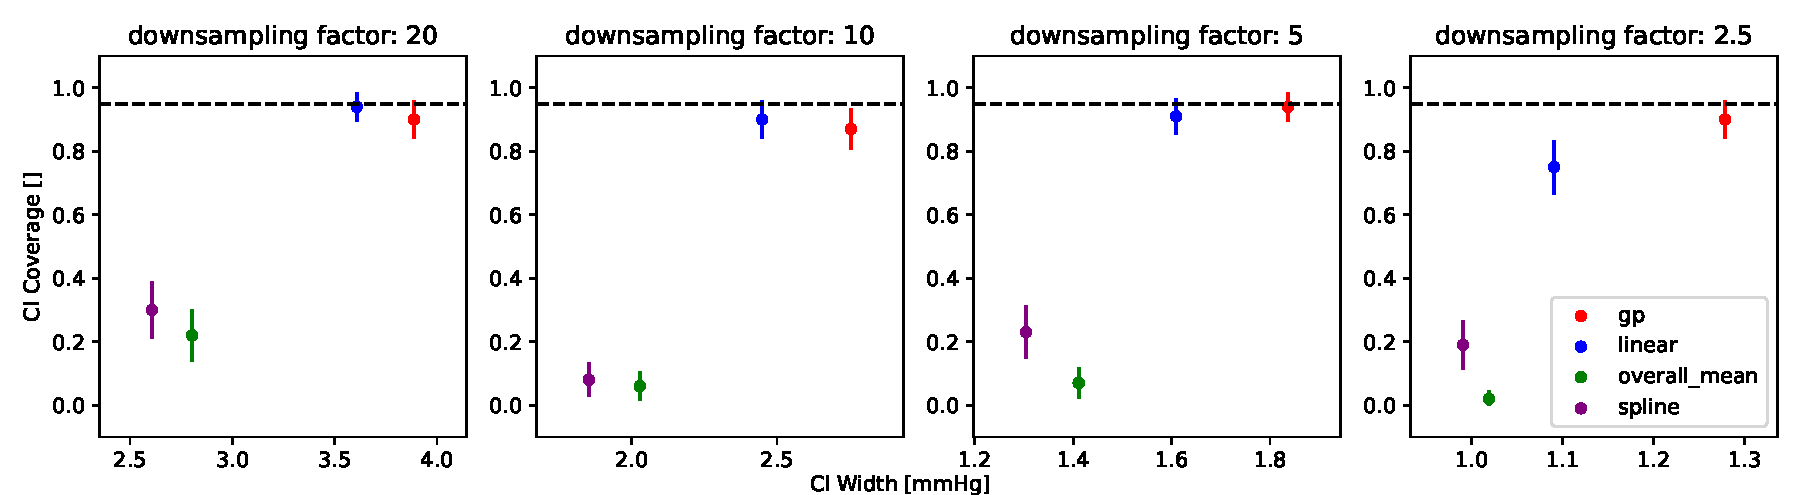
\includegraphics[width=\linewidth]{Pictures/final_experiment_hpdi/overall_mean_eval_sin_rbf_seasonal_default}
    \caption{One-Week Mean - Seasonal Downsampling}
    \label{fig:weekly-mean-seasonal-sampling-performance}
\end{subfigure}
\caption[One-Week Mean Performance]{The Performance of different methods to
estimate the one-week mean based on different downsampling patterns.
}
\label{fig:weekly-mean-performance}
\end{figure}



\section{One-Day and One-Hour Mean}

Figure \ref{fig:daily-mean-performance} and figure \ref{fig:daily-mean-performance}
show the Performance of different methods to
estimate the one-day and one-hour mean based on different downsampling patterns.



\begin{figure}[!ht]
\centering
\begin{subfigure}{\textwidth}
    \centering
    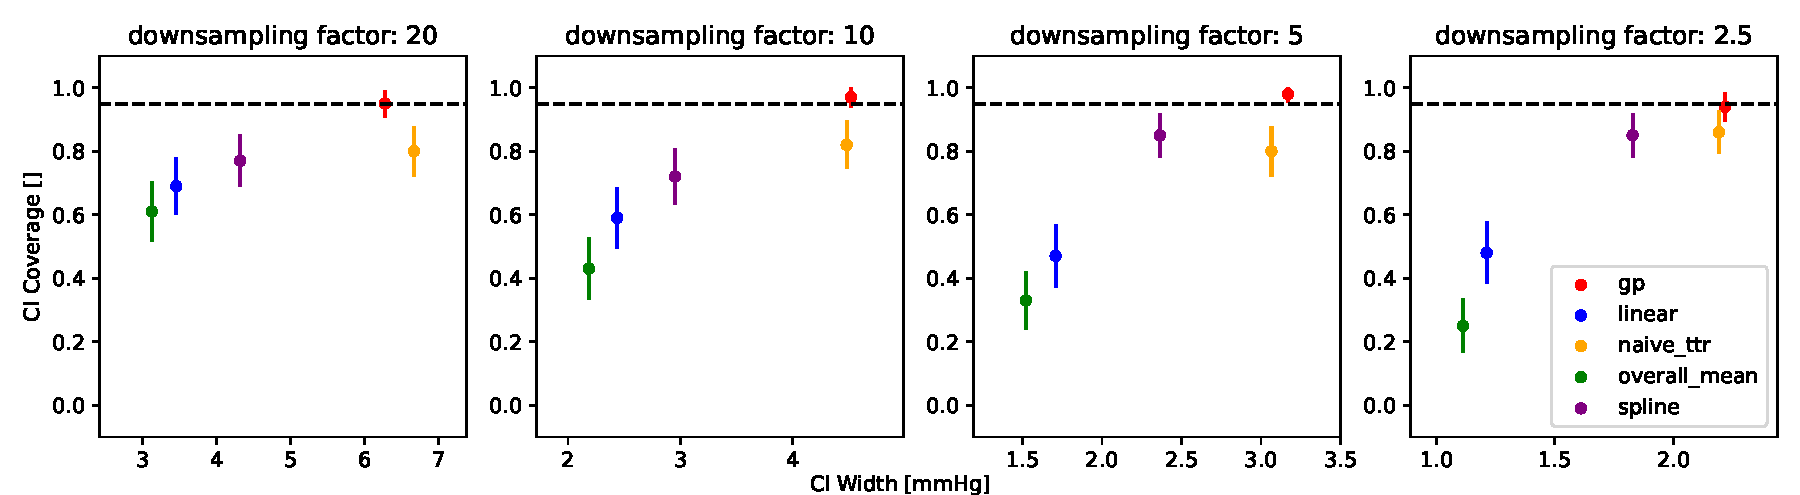
\includegraphics[width=\linewidth]{Pictures/final_experiment_hpdi/mean_24h_eval_sin_rbf_default}
    \caption{One-Day Mean Performance - Uniform Downsampling}
    \label{fig:daily-mean-uniform-sampling-performance}
\end{subfigure}

\bigskip

\begin{subfigure}{\textwidth}
    \centering
    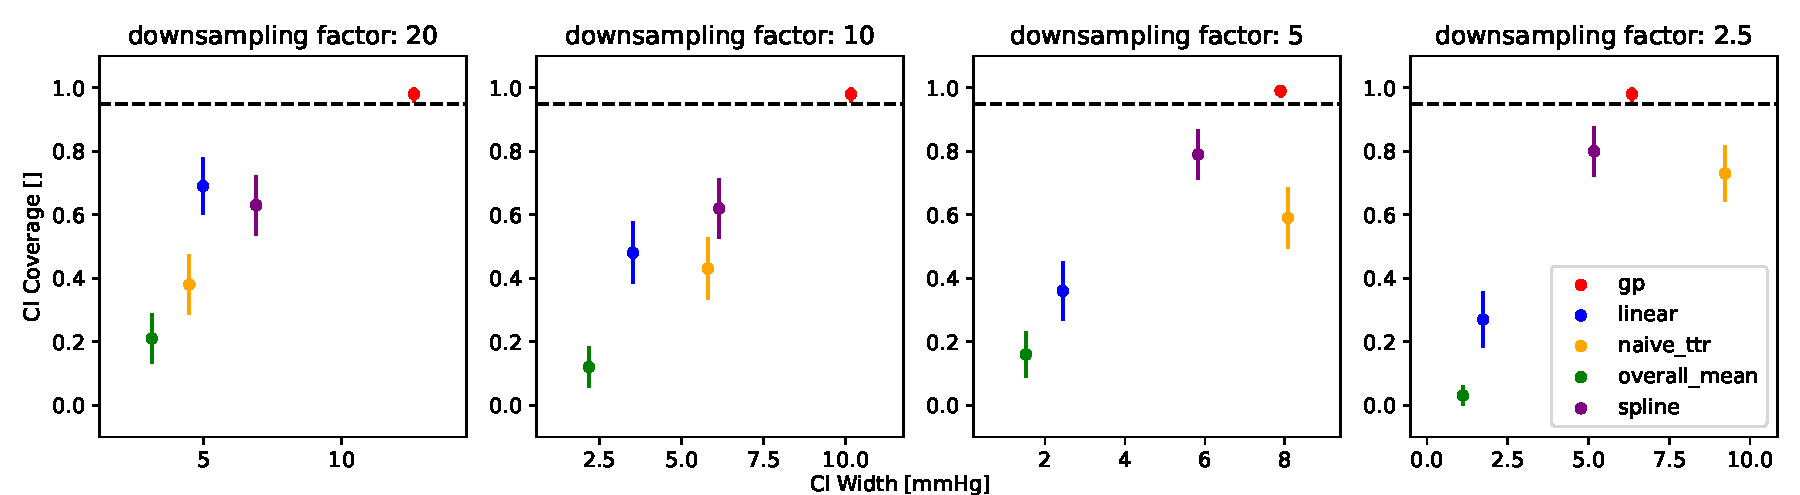
\includegraphics[width=\linewidth]{Pictures/final_experiment_hpdi/mean_1h_eval_sin_rbf_default}
    \caption{One-Day Mean Performance - Seasonal Downsampling}
    \label{fig:daily-mean-seasonal-sampling-performance}
\end{subfigure}
\caption[One-Day Mean Performance]{The Performance of different methods to
estimate the one-day mean based on different downsampling patterns.
}
\label{fig:daily-mean-performance}
\end{figure}




\begin{figure}[!ht]
\centering
\begin{subfigure}{\textwidth}
    \centering
    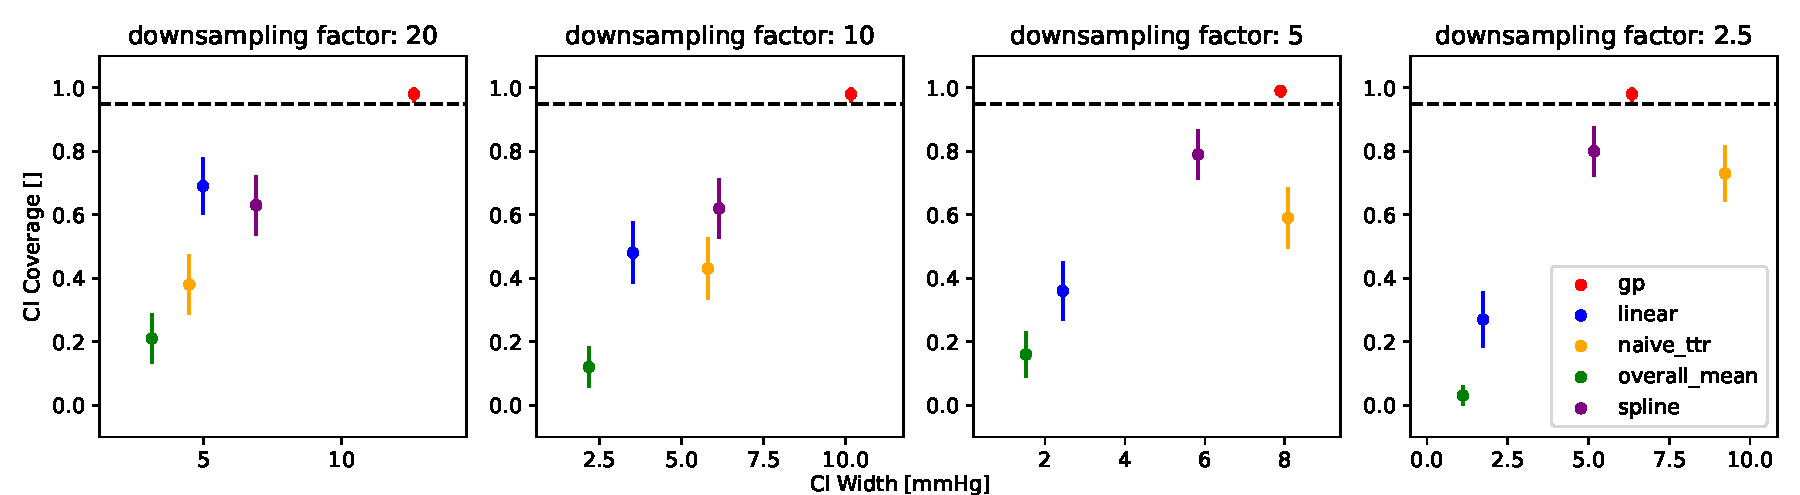
\includegraphics[width=\linewidth]{Pictures/final_experiment_hpdi/mean_1h_eval_sin_rbf_default}
    \caption{One-Hour Mean Performance - Uniform Downsampling}
    \label{fig:hourly-mean-uniform-sampling-performance}
\end{subfigure}

\bigskip

\begin{subfigure}{\textwidth}
    \centering
    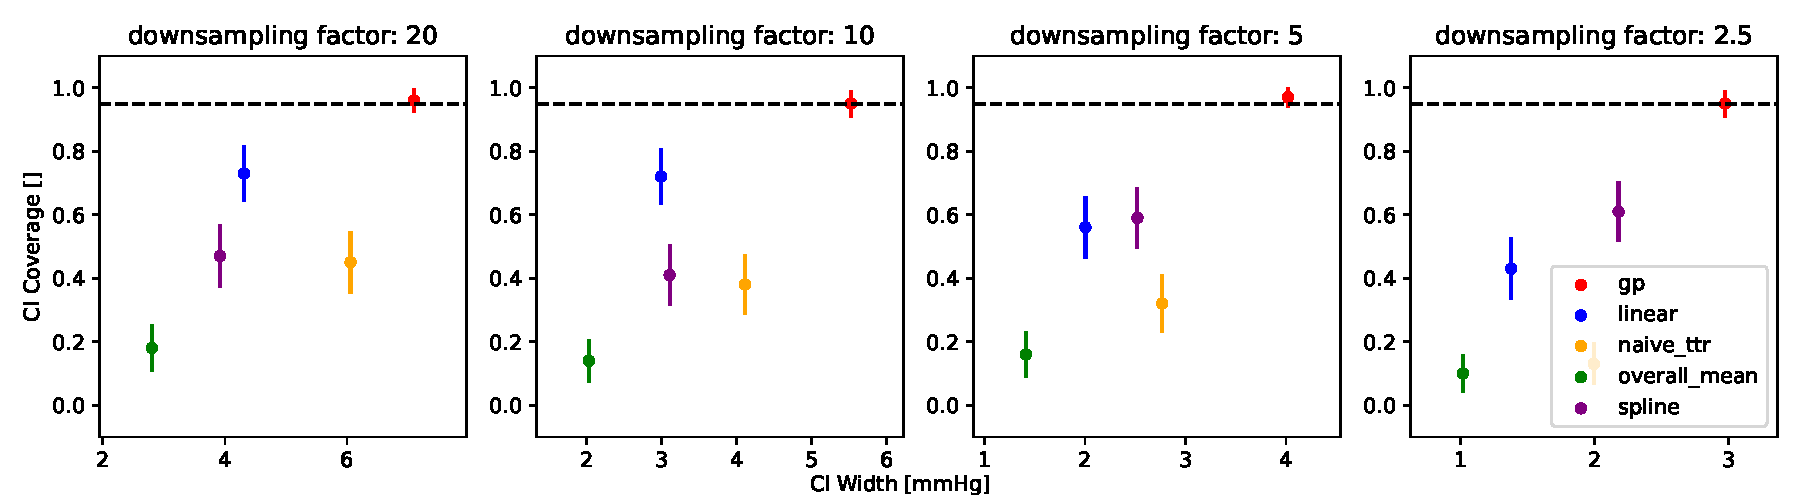
\includegraphics[width=\linewidth]{Pictures/final_experiment_hpdi/mean_24h_eval_sin_rbf_seasonal_default}
    \caption{One-Hour Mean Performance - Seasonal Downsampling}
    \label{fig:hourly-mean-seasonal-sampling-performance}
\end{subfigure}
\caption[One-Hour Mean Performance]{The Performance of different methods to
estimate the one-hour mean based on different downsampling patterns.
}
\label{fig:hourly-mean-performance}
\end{figure}


\section{Time in Target Range}

Figure \ref{fig:ttr-performance} shows the performance of different methods to
estimate time in target range (TTR) based on different downsampling patterns.
The only methods which sometimes reach the 95\% coverage target are
GP regression and smoothing spline interpolation, whereas GP regression produces
consistently lower CI width and does approach the target coverage with more
data.
Note that TTR does not care about the absolute values of the BP estimates
but does only check whether they are within the target range.
Since TTR is not affected by the extreme estimate values
occasionally produced by smoothing spline interpolation,
spline interpolation produces reasonable TTR estimates.
The current approach used to estimate TTR (naive_ttr) performs very baldy.
This is since it does not estimate TTR through estimation of $f(x)$ but directly
works on the noisy measurements $Y(x)$. It will thus generally underestimate
TTR.


\begin{figure}[!ht]
\centering
\begin{subfigure}{\textwidth}
    \centering
    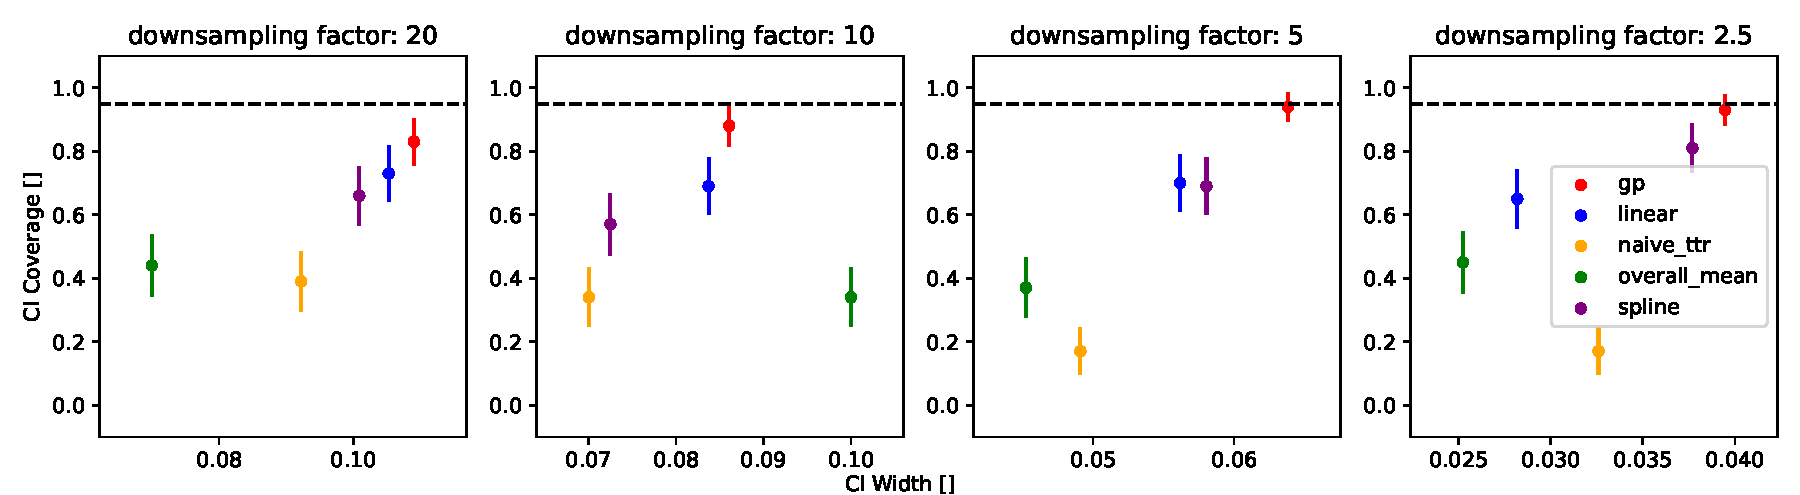
\includegraphics[width=\linewidth]{Pictures/final_experiment_hpdi/ttr_eval_sin_rbf_default}
    \caption{TTR Performance - Uniform Downsampling}
    \label{fig:ttr-uniform-sampling-performance}
\end{subfigure}

\bigskip

\begin{subfigure}{\textwidth}
    \centering
    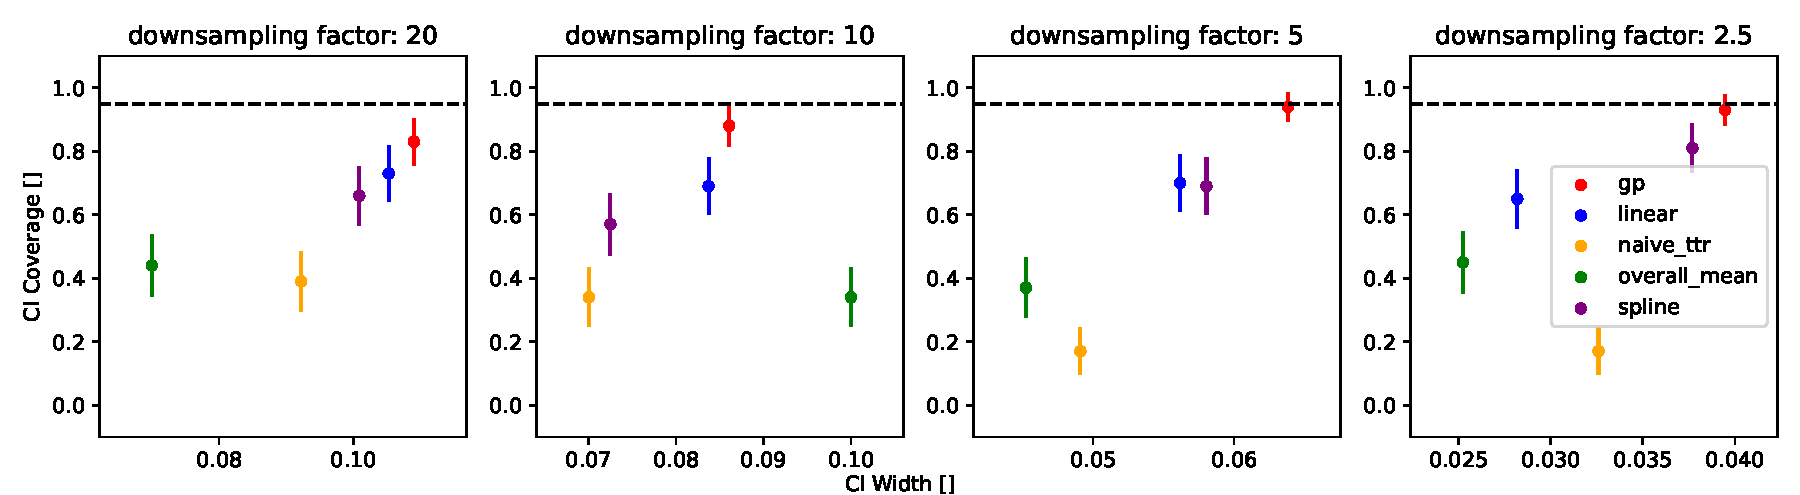
\includegraphics[width=\linewidth]{Pictures/final_experiment_hpdi/ttr_eval_sin_rbf_default}
    \caption{TTR Performance - Seasonal Downsampling}
    \label{fig:ttr-seasonal-sampling-performance}
\end{subfigure}
\caption[TTR Performance]{The Performance of different methods to
estimate TTR based on different downsampling patterns.
}
\label{fig:ttr-performance}
\end{figure}





\section{Examples}


\subsection{Pronounced Cyclic Component}

\begin{figure}[!ht]
\centering
    \includegraphics[width=\linewidth]{Pictures/plots_final3/sin_rbf_default_0.2/09_11_09_05_45/plot_mean_decomposed_vertical}
\caption[Decomposed BP time sereis]{Left panel: Decomposition of the true BP time series $f(x)$. Right panel:
Decomposition of $\hat{f})x$ estimated using GP regression.}
\label{fig:ex1-gp-prediction}
\end{figure}

\begin{figure}[!ht]
\centering

\begin{subfigure}{.45\textwidth}
    \centering
    \includegraphics[width=\linewidth]{Pictures/plots_final3/sin_rbf_default_0.2/09_11_09_05_45/plot_posterior_spline}
  \caption[Spline]{Smoothing spline prediction}
  \label{fig:ex1-spline}
\end{subfigure}\hfill
\begin{subfigure}{.45\textwidth}
    \centering
    \includegraphics[width=\linewidth]{Pictures/plots_final3/sin_rbf_default_0.2/09_11_09_05_45/plot_posterior_linear}
  \caption[Linear Regression]{Linear regression prediction}
  \label{fig:ex1-linear}
\end{subfigure}
\begin{subfigure}{0.6\textwidth}
    \centering
    \includegraphics[width=\linewidth]{Pictures/plots_final3/sin_rbf_default_0.2/09_11_09_05_45/plot_posterior}
  \caption[GP Prediction]{GP Regression prediciton with predictive variance (gray area)}
  \label{fig:ex1-spline}
\end{subfigure}
\caption[True BP value prediction]{Prediction of true BP values $F_X$ (black) form measurments (red dots). The true BP values are shown
by the red dotted line. }
\label{fig:ex1}
\end{figure}


\subsection{Pronounced AR Component}

\begin{figure}[!ht]
\centering
    \includegraphics[width=\linewidth]{Pictures/plots_final3/sin_rbf_default_0.2/09_11_09_05_07/plot_mean_decomposed_vertical}
\caption[Decomposed BP time sereis]{Left panel: Decomposition of the true BP time series $f(x)$. Right panel:
Decomposition of $\hat{f})x$ estimated using GP regression.}
\label{fig:ex2-gp-prediction}
\end{figure}

\begin{figure}[!ht]
\centering

\begin{subfigure}{.45\textwidth}
    \centering
    \includegraphics[width=\linewidth]{Pictures/plots_final3/sin_rbf_default_0.2/09_11_09_08_20/plot_posterior_spline}
  \caption[Spline]{Smoothing spline prediction}
  \label{fig:ex2-spline}
\end{subfigure}\hfill
\begin{subfigure}{.45\textwidth}
    \centering
    \includegraphics[width=\linewidth]{Pictures/plots_final3/sin_rbf_default_0.2/09_11_09_08_20/plot_posterior_linear}
  \caption[Linear Regression]{Linear regression prediction}
  \label{fig:ex2-linear}
\end{subfigure}
\begin{subfigure}{0.6\textwidth}
    \centering
    \includegraphics[width=\linewidth]{Pictures/plots_final3/sin_rbf_default_0.2/09_11_09_08_20/plot_posterior}
  \caption[GP Prediction]{GP Regression prediciton with predictive variance (gray area)}
  \label{fig:ex2-gp}
\end{subfigure}
\caption[True BP value prediction]{Prediction of true BP values $F_X$ (black) form measurments (red dots). The true BP values are shown
by the red dotted line. }
\label{fig:ex2}
\end{figure}



\begin{figure}[!ht]
\centering
    \includegraphics[width=\linewidth]{Pictures/plots_final3/sin_rbf_default_0.2/09_11_09_05_07/plot_mean_decomposed_vertical}
\caption[Decomposed BP time sereis]{Left panel: Decomposition of the true BP time series $f(x)$. Right panel:
Decomposition of $\hat{f})x$ estimated using GP regression.}
\label{fig:ex2-gp-prediction}
\end{figure}

\begin{figure}[!ht]
\centering

\begin{subfigure}{.45\textwidth}
    \centering
    \includegraphics[width=\linewidth]{Pictures/plots_final3/sin_rbf_default_0.2/09_11_09_08_20/plot_posterior_spline}
  \caption[Spline]{Smoothing spline prediction}
  \label{fig:ex2-spline}
\end{subfigure}\hfill
\begin{subfigure}{.45\textwidth}
    \centering
    \includegraphics[width=\linewidth]{Pictures/plots_final3/sin_rbf_default_0.2/09_11_09_08_20/plot_posterior_linear}
  \caption[Linear Regression]{Linear regression prediction}
  \label{fig:ex2-linear}
\end{subfigure}
\begin{subfigure}{0.6\textwidth}
    \centering
    \includegraphics[width=\linewidth]{Pictures/plots_final3/sin_rbf_default_0.2/09_11_09_08_20/plot_posterior}
  \caption[GP Prediction]{GP Regression prediciton with predictive variance (gray area)}
  \label{fig:ex2-gp}
\end{subfigure}
\caption[True BP value prediction]{Prediction of true BP values $F_X$ (black) form measurments (red dots). The true BP values are shown
by the red dotted line. }
\label{fig:ex2}
\end{figure}




\chapter{Discussion}
\section{Smoothing Spline Failure}

\begin{figure}[!ht]
\centering
\includegraphics[width=\linewidth]{Pictures/spline_extreme/plot_pred_bootstrap_spline_reg_v2_30}
\caption[Smoothing Spline Failure]{Smoothing Spline estimates of $F_X$ (black line)
    from bootsrap samples (red dots). The huge drop produced at the end of the one week window
    leads to very distorted overall mean estimates.}
\label{fig:ex2-gp-prediction}
\end{figure}






%\begin{example}
%
%\begin{figure}[!ht]
%\centering
%\includegraphics[width=\linewidth]{Pictures/plots_final2/sin_rbf_default_0.2/09_11_07_49_51/plot_posterior}
%\caption[GP Prediction]{Predictive mean of $F_{X}$ (blackline) with
%predictive variance (grey area) based on observations (red dots) }
%\label{fig:ex1-gp-prediction}
%\end{figure}
%
%\begin{figure}[!ht]
%\centering
%\includegraphics[width=\linewidth]{Pictures/plots_final2/sin_rbf_default_0.2/09_11_07_49_51/plot_mean_decomposed}
%\caption[Mean Decomposed Predicted vs True]{Each figure shows one sample $F_X$ drawn from the true GP (red dashed line) with noisy observations
%  (red dots) sampled at a frequency of 0.5/hour}
%\label{fig:ex1-gp-mean-decomposed}
%\end{figure}
%
%
%\begin{figure}[!ht]
%\centering
%\begin{subfigure}{.45\textwidth}
%    \centering
%    \includegraphics[width=\linewidth]{Pictures/plots_final2/sin_rbf_default_0.2/09_11_07_49_51/plot_posterior_spline}
%  \caption[Spline]{The sample $F_X$ shown to the right, decomposed in to the contribution of the Periodic kernel (orange),
%      Matérn kernel (blue), RBF kernel (green).}
%  \label{fig:ex1-spline}
%\end{subfigure}\hfill
%\begin{subfigure}{.45\textwidth}
%    \centering
%    \includegraphics[width=\linewidth]{Pictures/plots_final2/sin_rbf_default_0.2/09_11_07_49_51/plot_posterior_linear}
%  \caption[Linear Regression]{Each figure shows one sample $F_X$ drawn from the true GP (red dashed line) with noisy observations
%      (red dots) sampled at a frequency of 0.5/hour}
%  \label{fig:ex1-linear}
%\end{subfigure}
%\caption[Baseline Methods]{Baseline Methods Example Prediction}
%\label{fig:ex1}
%\end{figure}
%



%\end{example}









